\documentclass[11pt,a4paper]{article}

% ==========================================================
% Packages
% ==========================================================
\usepackage[margin=2.35cm]{geometry}
\usepackage[T1]{fontenc}
\usepackage[utf8]{inputenc}
\usepackage{lmodern}

\usepackage{amsmath, amssymb, bm}
\usepackage{graphicx}
\usepackage{booktabs}
\usepackage{array}
\usepackage{float}
\usepackage{xcolor}
\usepackage[hidelinks]{hyperref}
\usepackage{caption}
\usepackage{enumitem}

\graphicspath{{../plots/}{plots/}}

\setlength{\parindent}{0pt}
\setlength{\parskip}{6pt}

\captionsetup{
    font=small,
    labelfont=bf
}

% ==========================================================
% Title
% ==========================================================
\title{
    \textbf{Neural PDE Surrogate Benchmark}\\
    \large A Configurable PyTorch Benchmark for 1D and 2D Heat-Equation Surrogate Modelling
}
\date{}



\begin{document}

\maketitle

\begin{abstract}
This report describes a compact scientific machine learning benchmark for surrogate modelling of one-dimensional and two-dimensional heat-equation simulations. The project follows the full workflow from physics-based simulation to neural surrogate training: finite-difference solvers are used to generate supervised datasets, and PyTorch models are trained to predict final temperature fields from initial temperature fields and diffusion coefficients. Three model families are compared: multilayer perceptrons (MLPs), convolutional neural networks (CNNs), and Fourier Neural Operator-style (FNO-style) models.

The models are evaluated on both in-distribution test data and out-of-distribution (OOD) diffusion coefficients. In the 1D benchmark, the FNO-style model achieves the best performance with a test relative \(L^2\) error of \(0.30\%\) and an OOD relative \(L^2\) error of \(3.01\%\). In the 2D benchmark, the FNO-style model again performs best, with a test relative \(L^2\) error of \(0.45\%\) and an OOD relative \(L^2\) error of \(3.45\%\). The project shows how architecture choice, spatial inductive bias, and OOD evaluation matter in scientific ML surrogate modelling.
\end{abstract}



% ==========================================================
\section{Introduction}

Many scientific and engineering problems are studied using numerical simulation. These simulations are useful because they allow physical systems to be studied under different parameters, geometries, and boundary conditions. However, repeatedly running a numerical solver can become expensive, especially when many parameter combinations need to be explored.

A surrogate model is a machine learning model trained to approximate the input-output behaviour of a numerical solver. Once trained, the surrogate can produce approximate predictions much faster than repeatedly running the full simulation. In practical scientific workflows, surrogate models can support parameter studies, optimization, uncertainty analysis, active learning, and early-stage design exploration.

The goal of this project is to build a small but complete scientific ML benchmark around this idea. Instead of starting from a very complex simulator, the project uses the heat equation. The heat equation is simple enough to derive and understand clearly, but it still produces field-valued data. This makes it a useful benchmark for learning how to connect numerical simulation with neural surrogate modelling.

The complete workflow is:
\begin{equation}
    \text{PDE}
    \rightarrow
    \text{finite-difference solver}
    \rightarrow
    \text{simulation dataset}
    \rightarrow
    \text{neural surrogate models}
    \rightarrow
    \text{ID/OOD evaluation}.
\end{equation}

The project was first developed for the 1D heat equation and then extended to the 2D heat equation. The final implementation is organized as a configurable Python package. A user can select the problem dimension and model type from the command line, for example:
\begin{verbatim}
python -m neural_pde.generate_data --dim 1
python -m neural_pde.generate_data --dim 2
python -m neural_pde.train --dim 2 --model fno
python -m neural_pde.compare --dim 2
\end{verbatim}

This structure makes the benchmark easier to reproduce, extend, and present as a scientific ML portfolio project.

% ==========================================================
\section{Problem Formulation}

\subsection{Heat equation}

The heat equation describes diffusion of temperature over time. In compact notation, it is written as
\begin{equation}
    \frac{\partial u}{\partial t}
    =
    \alpha \nabla^2 u,
    \label{eq:heat_general}
\end{equation}
where \(u\) is the temperature field, \(t\) is time, \(\alpha\) is the diffusion coefficient, and \(\nabla^2\) is the Laplacian operator.

For the one-dimensional case, the equation becomes
\begin{equation}
    \frac{\partial u}{\partial t}
    =
    \alpha
    \frac{\partial^2 u}{\partial x^2}.
    \label{eq:heat_1d}
\end{equation}

For the two-dimensional case, the equation becomes
\begin{equation}
    \frac{\partial u}{\partial t}
    =
    \alpha
    \left(
    \frac{\partial^2 u}{\partial x^2}
    +
    \frac{\partial^2 u}{\partial y^2}
    \right).
    \label{eq:heat_2d}
\end{equation}

The diffusion coefficient \(\alpha\) controls how quickly heat spreads. A smaller value of \(\alpha\) produces slower smoothing, while a larger value produces stronger diffusion over the same simulation time.

\subsection{Surrogate learning task}

The supervised learning task is to approximate the mapping
\begin{equation}
    \mathcal{G}: (u_0, \alpha) \mapsto u_T,
    \label{eq:true_operator}
\end{equation}
where \(u_0\) is the initial temperature field and \(u_T\) is the final temperature field at time \(T\).

The neural network approximation is denoted by
\begin{equation}
    \mathcal{G}_{\theta}(u_0, \alpha) \approx u_T,
    \label{eq:learned_operator}
\end{equation}
where \(\theta\) represents the trainable model parameters.

In the 1D benchmark,
\begin{equation}
    u_0, u_T \in \mathbb{R}^{128}.
\end{equation}

In the 2D benchmark,
\begin{equation}
    u_0, u_T \in \mathbb{R}^{32 \times 32}.
\end{equation}

The model therefore learns a field-to-field mapping, not only a scalar regression problem.

% ==========================================================
\section{Boundary Conditions and Initial Conditions}

\subsection{Boundary conditions}

The project uses homogeneous Dirichlet boundary conditions. In simple terms, the boundary temperature is fixed to zero throughout the simulation.

For 1D, the domain is \(x \in [0,L]\), and the boundary conditions are
\begin{equation}
    u(0,t) = 0,
    \qquad
    u(L,t) = 0.
\end{equation}

For 2D, the square domain is \((x,y) \in [0,L] \times [0,L]\), and the boundary conditions are
\begin{align}
    u(0,y,t) &= 0,
    &
    u(L,y,t) &= 0,\\
    u(x,0,t) &= 0,
    &
    u(x,L,t) &= 0.
\end{align}

Physically, this can be interpreted as the boundary being connected to a cold reservoir. Numerically, it also gives a simple and stable benchmark setup.

\subsection{Random initial conditions}

The initial conditions are generated from smooth Gaussian bumps. For 1D, the initial field has the form
\begin{equation}
    u_0(x)
    =
    \sum_{k=1}^{K}
    A_k
    \exp
    \left(
    -
    \frac{(x-c_k)^2}{w_k}
    \right),
    \label{eq:initial_1d}
\end{equation}
where \(A_k\) is the amplitude, \(c_k\) is the centre, and \(w_k\) controls the width of the \(k\)-th bump.

For 2D, the initial field is generated as
\begin{equation}
    u_0(x,y)
    =
    \sum_{k=1}^{K}
    A_k
    \exp
    \left(
    -
    \frac{(x-c_{x,k})^2 + (y-c_{y,k})^2}{w_k}
    \right).
    \label{eq:initial_2d}
\end{equation}

These initial conditions create localized hot regions that then diffuse over time. This makes the learning task visually and physically interpretable.

% ==========================================================
\section{Finite-Difference Simulation}

The simulation labels are generated using explicit finite-difference methods. This section derives the update equations used in the code.

\subsection{1D finite-difference method}

For the 1D heat equation,
\begin{equation}
    \frac{\partial u}{\partial t}
    =
    \alpha
    \frac{\partial^2 u}{\partial x^2},
\end{equation}
the spatial domain is discretized using grid points
\begin{equation}
    x_i = i\Delta x,
    \qquad
    i = 0,1,\ldots,N_x-1.
\end{equation}

Time is discretized as
\begin{equation}
    t^n = n\Delta t.
\end{equation}

The numerical approximation is written as
\begin{equation}
    u_i^n \approx u(x_i,t^n).
\end{equation}

The time derivative is approximated using a forward difference:
\begin{equation}
    \frac{\partial u}{\partial t}
    \approx
    \frac{u_i^{n+1} - u_i^n}{\Delta t}.
\end{equation}

The second spatial derivative is approximated using a central difference:
\begin{equation}
    \frac{\partial^2 u}{\partial x^2}
    \approx
    \frac{
    u_{i-1}^{n}
    -
    2u_i^{n}
    +
    u_{i+1}^{n}
    }{\Delta x^2}.
\end{equation}

Substituting these approximations gives
\begin{equation}
    \frac{u_i^{n+1} - u_i^n}{\Delta t}
    =
    \alpha
    \frac{
    u_{i-1}^{n}
    -
    2u_i^{n}
    +
    u_{i+1}^{n}
    }{\Delta x^2}.
\end{equation}

Solving for \(u_i^{n+1}\) gives the update rule
\begin{equation}
    u_i^{n+1}
    =
    u_i^n
    +
    r
    \left(
    u_{i-1}^{n}
    -
    2u_i^{n}
    +
    u_{i+1}^{n}
    \right),
    \label{eq:fdm_1d}
\end{equation}
where
\begin{equation}
    r =
    \frac{\alpha \Delta t}{\Delta x^2}.
    \label{eq:r_1d}
\end{equation}

The number \(r\) is the diffusion number. For the explicit 1D heat-equation scheme, a common stability condition is
\begin{equation}
    r \leq \frac{1}{2}.
\end{equation}

In the code, only the interior points are updated. The two boundary values are reset to zero after each time step.

\subsection{1D numerical example}

Consider a small 1D grid with five points:
\begin{equation}
    u^n = [0,\;0.2,\;1.0,\;0.2,\;0].
\end{equation}

Let \(r=0.1\). The centre point is hot. Updating the centre point gives
\begin{equation}
    u_2^{n+1}
    =
    1.0
    +
    0.1(0.2 - 2(1.0) + 0.2)
    =
    0.84.
\end{equation}

The neighbouring points increase:
\begin{align}
    u_1^{n+1}
    &=
    0.2 + 0.1(0 - 2(0.2) + 1.0)
    =
    0.26,\\
    u_3^{n+1}
    &=
    0.2 + 0.1(1.0 - 2(0.2) + 0)
    =
    0.26.
\end{align}

So after one time step,
\begin{equation}
    u^{n+1} = [0,\;0.26,\;0.84,\;0.26,\;0].
\end{equation}

The centre value decreases and the neighbouring values increase. This is the basic mechanism of diffusion.

\subsection{2D finite-difference method}

For the 2D heat equation,
\begin{equation}
    \frac{\partial u}{\partial t}
    =
    \alpha
    \left(
    \frac{\partial^2 u}{\partial x^2}
    +
    \frac{\partial^2 u}{\partial y^2}
    \right),
\end{equation}
a rectangular grid is used. Let
\begin{equation}
    u_{j,i}^{n} \approx u(x_i,y_j,t^n).
\end{equation}

Assuming \(\Delta x = \Delta y\), the 2D Laplacian is approximated using the standard five-point stencil:
\begin{equation}
    \nabla^2 u
    \approx
    \frac{
    u_{j,i-1}^{n}
    +
    u_{j,i+1}^{n}
    +
    u_{j-1,i}^{n}
    +
    u_{j+1,i}^{n}
    -
    4u_{j,i}^{n}
    }{\Delta x^2}.
\end{equation}

Therefore, the 2D update rule is
\begin{equation}
    u_{j,i}^{n+1}
    =
    u_{j,i}^{n}
    +
    r
    \left(
    u_{j,i-1}^{n}
    +
    u_{j,i+1}^{n}
    +
    u_{j-1,i}^{n}
    +
    u_{j+1,i}^{n}
    -
    4u_{j,i}^{n}
    \right),
    \label{eq:fdm_2d}
\end{equation}
where
\begin{equation}
    r =
    \frac{\alpha \Delta t}{\Delta x^2}.
\end{equation}

For the explicit 2D heat-equation scheme, the stability condition is stricter:
\begin{equation}
    r \leq \frac{1}{4}.
\end{equation}

In the code, the four boundaries of the 2D grid are fixed to zero after every update.

\subsection{2D numerical example}

Consider a small \(5 \times 5\) grid where only the centre point is hot:
\begin{equation}
u^n =
\begin{bmatrix}
0 & 0 & 0 & 0 & 0\\
0 & 0 & 0 & 0 & 0\\
0 & 0 & 1 & 0 & 0\\
0 & 0 & 0 & 0 & 0\\
0 & 0 & 0 & 0 & 0
\end{bmatrix}.
\end{equation}

Let \(r=0.1\). The centre point is updated as
\begin{equation}
    u_{2,2}^{n+1}
    =
    1 + 0.1(0+0+0+0-4)
    =
    0.6.
\end{equation}

The four direct neighbours receive heat from the centre, so after one time step the grid becomes
\begin{equation}
u^{n+1} =
\begin{bmatrix}
0 & 0 & 0 & 0 & 0\\
0 & 0 & 0.1 & 0 & 0\\
0 & 0.1 & 0.6 & 0.1 & 0\\
0 & 0 & 0.1 & 0 & 0\\
0 & 0 & 0 & 0 & 0
\end{bmatrix}.
\end{equation}

This example shows the same diffusion idea as in 1D, but now heat spreads in both coordinate directions.

% ==========================================================
\section{Dataset Generation}

The solver is used to generate supervised learning data. For each sample, the code performs the following steps:
\begin{enumerate}[leftmargin=*]
    \item sample a diffusion coefficient \(\alpha\),
    \item generate a random smooth initial field \(u_0\),
    \item evolve the heat equation using the finite-difference solver,
    \item save the final field \(u_T\) as the target.
\end{enumerate}

The dataset splits are shown in Table~\ref{tab:dataset_splits}.

\begin{table}[H]
    \centering
    \caption{Dataset splits used in the benchmark.}
    \label{tab:dataset_splits}
    \begin{tabular}{lccc}
        \toprule
        Split & Samples & Diffusion coefficient range & Purpose \\
        \midrule
        Train & 2000 & \(0.005\)--\(0.030\) & Model training \\
        Validation & 300 & \(0.005\)--\(0.030\) & Checkpoint selection \\
        Test & 300 & \(0.005\)--\(0.030\) & In-distribution evaluation \\
        OOD test & 300 & \(0.035\)--\(0.060\) & Out-of-distribution evaluation \\
        \bottomrule
    \end{tabular}
\end{table}

The OOD set uses larger diffusion coefficients than the training set. This means the model must predict stronger smoothing behaviour than it directly observed during training.

The array shapes are shown in Table~\ref{tab:data_shapes}.

\begin{table}[H]
    \centering
    \caption{Dataset array shapes.}
    \label{tab:data_shapes}
    \begin{tabular}{lccc}
        \toprule
        Benchmark & \(u_0\) shape & \(\alpha\) shape & \(u_T\) shape \\
        \midrule
        1D heat equation & \((N,128)\) & \((N,1)\) & \((N,128)\) \\
        2D heat equation & \((N,32,32)\) & \((N,1)\) & \((N,32,32)\) \\
        \bottomrule
    \end{tabular}
\end{table}

% ==========================================================
\section{Neural Surrogate Models}

Three model families are used in this benchmark. The point of comparing them is not only to get the lowest error, but also to understand how different architectural assumptions affect scientific ML performance.

\subsection{MLP baseline}

The multilayer perceptron is the simplest baseline. It receives a flattened field and the diffusion coefficient. For 1D, the input dimension is
\begin{equation}
    128 + 1 = 129.
\end{equation}

For 2D, the input dimension is
\begin{equation}
    32 \times 32 + 1 = 1025.
\end{equation}

A hidden layer of an MLP can be written as
\begin{equation}
    \bm{h}^{(\ell+1)}
    =
    \sigma
    \left(
    W^{(\ell)}
    \bm{h}^{(\ell)}
    +
    \bm{b}^{(\ell)}
    \right),
\end{equation}
where \(W^{(\ell)}\) is a weight matrix, \(\bm{b}^{(\ell)}\) is a bias vector, and \(\sigma\) is a nonlinear activation.

The MLP is useful because it gives a basic reference point. However, it does not explicitly know that neighbouring grid points are physically related. This becomes especially limiting in the 2D benchmark.

\subsection{CNN surrogate}

CNNs use local filters and parameter sharing. This is useful for physical fields because heat diffusion is local: each point is influenced by nearby points.

For a 1D convolution, the operation can be written as
\begin{equation}
    y_o[j]
    =
    \sum_c
    \sum_k
    w_{o,c,k}
    x_c[j+k]
    +
    b_o.
\end{equation}

For a 2D convolution, the operation becomes
\begin{equation}
    y_o[p,q]
    =
    \sum_c
    \sum_{a,b}
    w_{o,c,a,b}
    x_c[p+a,q+b]
    +
    b_o.
\end{equation}

The CNN input contains two channels:
\begin{itemize}[leftmargin=*]
    \item the initial field \(u_0\),
    \item the normalized diffusion coefficient \(\alpha\), repeated over the grid.
\end{itemize}

Repeating \(\alpha\) gives every spatial location access to the diffusion strength.

\subsection{FNO-style surrogate}

The FNO-style model is designed around the idea of learning field-to-field mappings. Instead of only working with local spatial filters, it applies part of the transformation in Fourier space.

The spectral convolution follows this pattern:
\begin{equation}
    \text{physical field}
    \rightarrow
    \text{Fourier transform}
    \rightarrow
    \text{learned spectral weights}
    \rightarrow
    \text{inverse Fourier transform}.
\end{equation}

For a 1D spectral layer, the core operation is
\begin{equation}
    Y_{b,o,m}
    =
    \sum_i
    X_{b,i,m}
    W_{i,o,m},
    \label{eq:fno_1d}
\end{equation}
where \(b\) is the batch index, \(i\) is the input channel, \(o\) is the output channel, and \(m\) is the Fourier mode.

In the PyTorch implementation, this is written as
\begin{verbatim}
torch.einsum("bim,iom->bom", x_ft, weights)
\end{verbatim}

For the 2D case, the spectral weights operate over two Fourier-mode dimensions:
\begin{equation}
    Y_{b,o,k_x,k_y}
    =
    \sum_i
    X_{b,i,k_x,k_y}
    W_{i,o,k_x,k_y}.
    \label{eq:fno_2d}
\end{equation}

Fourier coefficients are complex-valued, so the spectral weights are also complex-valued. This allows the layer to learn transformations of both amplitude and phase information.

The heat equation is well suited to Fourier-based modelling because diffusion has a natural frequency interpretation. Sharp features correspond to higher-frequency components, and heat diffusion damps high-frequency components more strongly than low-frequency components.

% ==========================================================
\section{Training and Evaluation}

All models are trained using mean squared error loss:
\begin{equation}
    \mathcal{L}_{\text{MSE}}
    =
    \frac{1}{N}
    \sum_{i=1}^{N}
    (y_i - \hat{y}_i)^2.
\end{equation}

The Adam optimizer is used for training. The best model checkpoint is selected using validation loss.

The main evaluation metrics are mean squared error, mean absolute error, and relative \(L^2\) error.

\subsection{Mean squared error}

\begin{equation}
    \text{MSE}
    =
    \frac{1}{N}
    \sum_i
    (y_i - \hat{y}_i)^2.
\end{equation}

\subsection{Mean absolute error}

\begin{equation}
    \text{MAE}
    =
    \frac{1}{N}
    \sum_i
    |y_i - \hat{y}_i|.
\end{equation}

\subsection{Relative \(L^2\) error}

For field prediction tasks, relative \(L^2\) error is especially useful:
\begin{equation}
    \text{Relative } L^2
    =
    \frac{
    \lVert \bm{y} - \hat{\bm{y}} \rVert_2
    }{
    \lVert \bm{y} \rVert_2
    }.
\end{equation}

A relative \(L^2\) error of \(0.01\) corresponds approximately to a \(1\%\) relative error.

% ==========================================================
\section{Reproducibility Setup}

The benchmark is controlled using YAML configuration files. The main settings used for the experiments are summarized in Table~\ref{tab:reproducibility}.

\begin{table}[H]
    \centering
    \caption{Main reproducibility settings used in the benchmark.}
    \label{tab:reproducibility}
    \begin{tabular}{lll}
        \toprule
        Setting & 1D benchmark & 2D benchmark \\
        \midrule
        Grid size & \(128\) & \(32 \times 32\) \\
        Train / validation / test / OOD samples & \(2000/300/300/300\) & \(2000/300/300/300\) \\
        Training \(\alpha\) range & \(0.005\)--\(0.030\) & \(0.005\)--\(0.030\) \\
        OOD \(\alpha\) range & \(0.035\)--\(0.060\) & \(0.035\)--\(0.060\) \\
        Optimizer & Adam & Adam \\
        Loss & MSE & MSE \\
        Epochs & 80 & 80 \\
        Random seed & 42 & 42 \\
        \bottomrule
    \end{tabular}
\end{table}

Generated datasets and model checkpoints are intentionally excluded from git because they can be regenerated. Result tables, figures, source code, configuration files, and the report are included so that the repository remains lightweight but informative.

% ==========================================================
\section{Results}

\subsection{1D benchmark results}

The 1D results are shown in Table~\ref{tab:results_1d}.

\begin{table}[H]
    \centering
    \caption{1D heat-equation benchmark results.}
    \label{tab:results_1d}
    \begin{tabular}{lccc}
        \toprule
        Model & Test relative \(L^2\) & OOD relative \(L^2\) & Parameters \\
        \midrule
        MLP & \(1.54\%\) & \(5.47\%\) & \(197{,}760\) \\
        CNN1D & \(1.20\%\) & \(8.47\%\) & \(62{,}657\) \\
        FNO1D & \(\mathbf{0.30\%}\) & \(\mathbf{3.01\%}\) & \(287{,}489\) \\
        \bottomrule
    \end{tabular}
\end{table}

The CNN1D model improves the in-distribution test error compared with the MLP. However, it performs worse on the OOD diffusion range. This is an important result because it shows that better interpolation accuracy does not automatically imply better extrapolation.

The FNO1D model achieves the best performance on both test and OOD data. This supports the idea that Fourier-based representations are useful for diffusion problems.

\begin{figure}[H]
    \centering
    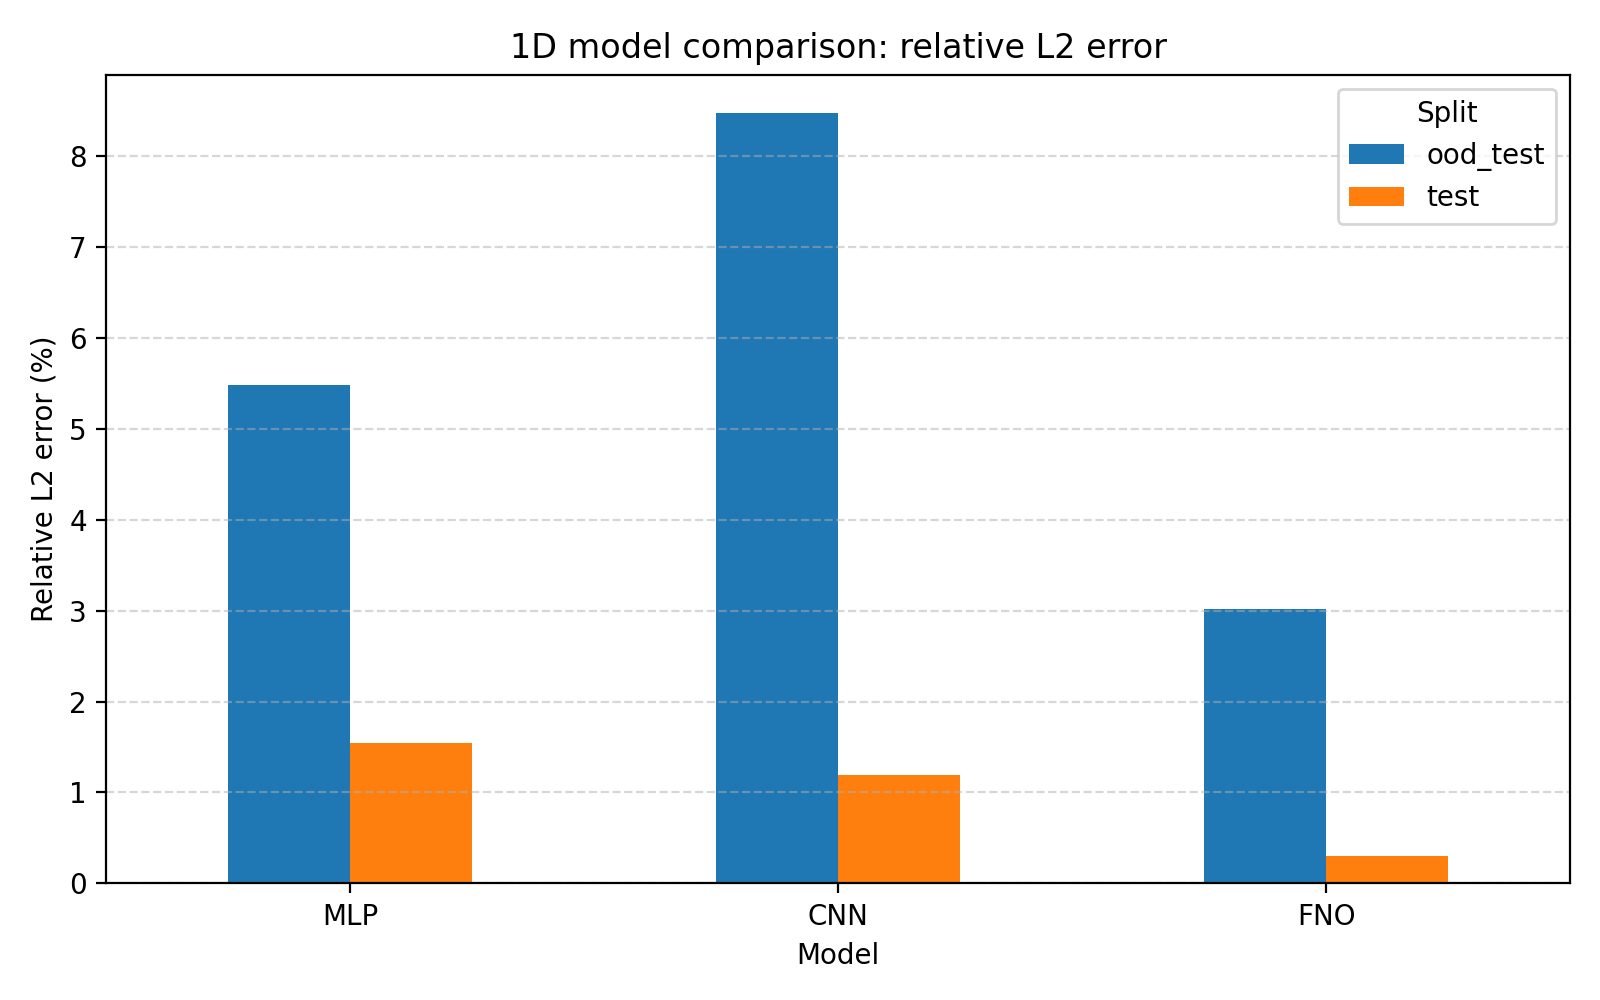
\includegraphics[width=0.82\textwidth]{heat1d/model_comparison_relative_l2.png}
    \caption{1D model comparison using relative \(L^2\) error for the in-distribution test set and OOD test set.}
    \label{fig:results_1d}
\end{figure}

\subsection{2D benchmark results}

The 2D results are shown in Table~\ref{tab:results_2d}.

\begin{table}[H]
    \centering
    \caption{2D heat-equation benchmark results.}
    \label{tab:results_2d}
    \begin{tabular}{lccc}
        \toprule
        Model & Test relative \(L^2\) & OOD relative \(L^2\) & Parameters \\
        \midrule
        MLP & \(6.83\%\) & \(6.90\%\) & \(1{,}575{,}936\) \\
        CNN2D & \(0.50\%\) & \(3.67\%\) & \(312{,}257\) \\
        FNO2D & \(\mathbf{0.45\%}\) & \(\mathbf{3.45\%}\) & \(1{,}188{,}385\) \\
        \bottomrule
    \end{tabular}
\end{table}

The MLP performs much worse in 2D, even though it has many parameters. This happens because flattening the 2D field removes the spatial structure from the model input. CNN2D and FNO2D perform much better because they preserve the field structure.

The FNO2D model gives the best overall result, although the improvement over CNN2D is smaller than in the 1D case. This is a useful observation: for this smooth 2D heat-equation task, a CNN already captures much of the local diffusion behaviour. The FNO-style model still performs best, but not by a large margin.

\begin{figure}[H]
    \centering
    
\includegraphics[width=0.82\textwidth]{heat2d/model_comparison_relative_l2.png}
    \caption{2D model comparison using relative \(L^2\) error for the in-distribution test set and OOD test set.}
    \label{fig:results_2d}
\end{figure}

\begin{figure}[H]
    \centering
    
\includegraphics[width=0.95\textwidth]{heat2d/fno_test_predictions.png}
    \caption{FNO2D prediction examples on in-distribution test data. Each row compares the initial field, the finite-difference target, and the neural surrogate prediction.}
    \label{fig:fno2d_test}
\end{figure}

\begin{figure}[H]
    \centering
    
\includegraphics[width=0.95\textwidth]{heat2d/fno_ood_predictions.png}
    \caption{FNO2D prediction examples on OOD diffusion coefficients. The examples show that the model still captures the main smoothing behaviour for larger unseen diffusion values.}
    \label{fig:fno2d_ood}
\end{figure}

% ==========================================================
\section{Discussion}

The results show several useful lessons.

First, the MLP baseline is helpful but limited. It can learn the 1D mapping reasonably well, but it struggles in the 2D benchmark. This is expected because the MLP treats the input as a flat vector and does not directly use spatial structure.

Second, CNN models are strong for field data. CNN1D improves the 1D test error compared with the MLP, and CNN2D performs much better than the 2D MLP. This confirms that local spatial inductive bias is important for PDE surrogate modelling.

Third, the CNN result also shows why OOD testing matters. In the 1D benchmark, CNN1D has better in-distribution error than the MLP but worse OOD error. If only the normal test set were used, this weakness would be missed.

Fourth, the FNO-style models perform best overall. The improvement is especially clear in 1D. In 2D, the FNO-style model is slightly better than CNN2D, but both models are strong. This is reasonable because the heat equation is smooth and local, so CNNs already perform well. The FNO-style model still has an advantage because it can learn global frequency-domain transformations.

The main conclusion is not simply that one model is always best. A better conclusion is that architecture choice must match the structure of the physical problem. For PDE surrogate modelling, it is useful to compare simple baselines, spatial models, and operator-inspired architectures under both in-distribution and OOD settings.

% ==========================================================
\section{Software Design}

The final project is organized as a configurable Python package. Instead of keeping separate scripts for every model and dimension, the code uses common training, evaluation, metric, and plotting utilities.

The main directory structure is:
\begin{verbatim}
configs/                    YAML experiment configurations
src/neural_pde/             main Python package
src/neural_pde/solvers/     finite-difference heat-equation solvers
src/neural_pde/models/      MLP, CNN, and FNO-style model definitions
data/                       generated datasets, ignored by git
checkpoints/                trained model checkpoints, ignored by git
results/                    metrics and comparison CSV files
plots/                      generated figures
reports/                    technical report
notes/                      project notes
\end{verbatim}

The workflow is controlled using command-line arguments:
\begin{verbatim}
python -m neural_pde.generate_data --dim 1
python -m neural_pde.generate_data --dim 2
python -m neural_pde.train --dim 1 --model mlp
python -m neural_pde.train --dim 1 --model cnn
python -m neural_pde.train --dim 1 --model fno
python -m neural_pde.train --dim 2 --model mlp
python -m neural_pde.train --dim 2 --model cnn
python -m neural_pde.train --dim 2 --model fno
python -m neural_pde.compare --dim 1
python -m neural_pde.compare --dim 2
\end{verbatim}

This design makes the project easier to reproduce and extend. For example, a new PDE, a new neural architecture, or a new OOD test can be added without rewriting the full training pipeline.

% ==========================================================
\section{Limitations}

This project is intentionally compact, so it has limitations:
\begin{itemize}[leftmargin=*]
    \item The heat equation is linear and smooth.
    \item The 2D grid is currently limited to \(32 \times 32\).
    \item Only one type of OOD shift is tested: larger diffusion coefficients.
    \item The FNO implementation is simplified and intended as a benchmark model, not a fully optimized research library.
    \item Uncertainty estimation is not included yet.
    \item Active learning is not included yet.
    \item Runtime speedup against the finite-difference solver is not yet benchmarked.
\end{itemize}

These limitations are useful because they suggest clear next steps for improving the project.

% ==========================================================
\section{Future Work}

The most useful future extensions are:
\begin{itemize}[leftmargin=*]
    \item increase the 2D grid resolution to \(64 \times 64\),
    \item add nonlinear PDEs such as Burgers' equation or reaction-diffusion systems,
    \item predict multiple future time steps instead of only one final state,
    \item add uncertainty estimation using model ensembles,
    \item add active learning for selecting new simulation points,
    \item benchmark neural surrogate inference time against the finite-difference solver,
    \item add additional OOD tests, such as sharper initial conditions or different boundary conditions.
\end{itemize}

A particularly important next step is runtime benchmarking, because one of the main reasons to use surrogate models is speed. Comparing finite-difference solver time with neural-network inference time would strengthen the engineering relevance of the project.

% ==========================================================
\section{Conclusion}

This project developed a configurable PyTorch benchmark for 1D and 2D PDE surrogate modelling using the heat equation. Finite-difference solvers were implemented to generate supervised simulation data, and three neural surrogate families were compared: MLP, CNN, and FNO-style models.

The FNO-style models achieved the best overall performance in both 1D and 2D benchmarks. In 1D, FNO1D reached \(0.30\%\) test relative \(L^2\) error and \(3.01\%\) OOD relative \(L^2\) error. In 2D, FNO2D reached \(0.45\%\) test relative \(L^2\) error and \(3.45\%\) OOD relative \(L^2\) error. CNN models also performed strongly, especially in 2D, while MLPs were useful baselines but weaker for structured field prediction.

The main lesson is that scientific ML surrogate models should be evaluated not only by test accuracy but also by their behaviour under OOD parameter shifts. The project also shows that architecture choice matters: spatial and spectral inductive biases can substantially improve field-to-field prediction.

% ==========================================================
\section*{References}
\addcontentsline{toc}{section}{References}

\begin{thebibliography}{9}

\bibitem{leveque2007}
R. J. LeVeque,
\textit{Finite Difference Methods for Ordinary and Partial Differential Equations},
SIAM, 2007.

\bibitem{goodfellow2016}
I. Goodfellow, Y. Bengio, and A. Courville,
\textit{Deep Learning},
MIT Press, 2016.

\bibitem{li2020fno}
Z. Li, N. Kovachki, K. Azizzadenesheli, B. Liu, K. Bhattacharya, A. Stuart, and A. Anandkumar,
``Fourier Neural Operator for Parametric Partial Differential Equations,''
arXiv:2010.08895, 2020.

\bibitem{lu2021deeponet}
L. Lu, P. Jin, G. Pang, Z. Zhang, and G. E. Karniadakis,
``Learning nonlinear operators via DeepONet based on the universal approximation theorem of operators,''
\textit{Nature Machine Intelligence}, 2021.

\bibitem{raissi2019pinn}
M. Raissi, P. Perdikaris, and G. E. Karniadakis,
``Physics-informed neural networks: A deep learning framework for solving forward and inverse problems involving nonlinear partial differential equations,''
\textit{Journal of Computational Physics}, 2019.

\end{thebibliography}

\end{document}
